
          %---------------------------------------------------%
\chapter{~~Quotient manifolds and periodic boundary conditions}
          %---------------------------------------------------%
\label{\numb section 7}


The roots of {\maniFEM} go back to a PhD thesis in 2002
% (or even earlier, to a Master thesis in 1997)
where finite elements on a torus were implemented in {\small\tt FORTRAN}.%
\footnote{See % C.~Barbarosie, Optimization of perforated domains through homogenization,
% Structural Optimization 14, 1997
C.~Barbarosie, Shape optimization of periodic structures,
Computers \& Structures 30, 2003}
The torus is meant as a mere quotient manifold between $ \mathbb{R}^2 $ and a group of
translations of $ \mathbb{R}^2 $ with two generators;
you may think of it as $ {\mathbb R}^2/{\mathbb Z}^2 $.
It should be stressed that this manifold is not the usual ``doughnut'' built in paragraph
\ref{\numb section 2.\numb parag 16}.
These two manifolds are homeomorphic (topologically equivalent) but they are not isometric,
that is, their geometry differ.
The quotient torus is a Riemann manifold with no curvature; it is locally Euclidian
(that is, locally isometric to open sets of $ \mathbb{R}^2 $); we may call it ``flat torus''.
It cannot be embedded in $ \mathbb{R}^3 $, much less be represented graphically.
An unfolded mesh in $ \mathbb{R}^2 $ can be represented graphically, where vertices and segments
from the torus are drawn more than once.

One of the goals of {\maniFEM} is to deal with meshes on quotient manifolds.
Different quotient operations can be used, with groups of translations of $ \mathbb{R}^2 $ but also
with other groups of transformations.


          %--------------------------%
\section{~~A circle with no curvature}\label{\numb section 7.\numb parag 1}
          %--------------------------%

Here is the closed curve $ \mathbb{R}/{\mathbb Z} $.
We define it as a segment from {\small\tt A} to {\small\tt A}, with a specified {\small\tt spin}.

\begin{Verbatim}[commandchars=\\\{\},formatcom=\small\tt,frame=single,
   label=parag-\ref{\numb section 7.\numb parag 2}.cpp,rulecolor=\color{coment},
   baselinestretch=0.94,framesep=2mm                                            ]
   \cinza{// begin with the one-dimensional line}
   \verm{Manifold} \azul{RR} ( \verm{tag}::Euclid, \verm{tag}::of_dim, 1 );
   \verm{Function} \azul{x} = RR.build_coordinate_system ( \verm{tag}::Lagrange, \verm{tag}::of_degree, 1 );

   \cinza{// define an action on RR (a translation)}
   \verm{Function}::Action \azul{g} ( tag::transforms, x, tag::into, x+1. );
   \verm{Manifold} \azul{circle} = RR.quotient ( g );

   \cinza{// one vertex is enough to start the process}
   \verm{Cell} \azul{A} ( \verm{tag}::vertex );  x(A) = 0.02;
   \cinza{// with this vertex, we build a segment}
   \verm{Mesh} \azul{seg} ( \verm{tag}::segment, A.reverse(), A, \verm{tag}::divided_in, 10, \verm{tag}::spin, g );
\end{Verbatim}

We do not bother with the graphical representation of this one-dimensional mesh.

This mesh has 10 segments and 10 vertices. It has no boundary.
In contrast, if we mesh a segment in the usual Euclidian space $ \mathbb{R} $,
we get 10 segments and 11 vertices (and we get a boundary made of two vertices).

In an effort not to expose too many names in the {\small\tt namespace \verm{maniFEM}},
we have chosen to hide the class name {\small\tt Action} inside the namespace of
{\small\tt class \verm{Function}}.
See paragraph \ref{\numb section 11.\numb parag 1}.


          %---------------%
\section{~~A curved circle}\label{\numb section 7.\numb parag 2}
          %---------------%

We are now in a position to resume the example in paragraph \ref{\numb section 2.\numb parag 15},
this time in a less cumbersome manner.

\begin{Verbatim}[commandchars=\\\{\},formatcom=\small\tt,frame=single,
   label=parag-\ref{\numb section 7.\numb parag 2}.cpp,rulecolor=\color{coment},
   baselinestretch=0.94,framesep=2mm                                            ]
   \verm{Manifold} \azul{RR} ( \verm{tag}::Euclid, \verm{tag}::of_dim, 1 );
   \verm{Function} \azul{theta} = RR.build_coordinate_system ( \verm{tag}::Lagrange, \verm{tag}::of_degree, 1 );
   const double \azul{pi} = 3.1415926536;
   \verm{Function}::Action \azul{g} ( tag::transforms, theta, tag::into, theta + 2*pi );
   \verm{Manifold} \azul{circle} = RR.quotient ( g );

   \verm{Cell} \azul{A} ( \verm{tag}::vertex );  theta ( A ) = 0.;
   \verm{Mesh} \azul{loop} ( \verm{tag}::segment, A.reverse(), A, \verm{tag}::divided_in, 20, \verm{tag}::spin, g );

   \cinza{// define new coordinates x and y as arithmetic expressions of theta}
   \verm{Function} \azul{x} = \verm{cos}(theta), \azul{y} = \verm{sin}(theta);
   \cinza{// forget about theta; in future statements, x and y will be used}
   circle.set_coordinates ( x && y );
   seg.export_msh (\verde{"circle.msh"});
\end{Verbatim}

In {\tt gmsh}, you must select {\small\tt Tools} $\to$ {\small\tt Options} $\to$
{\small\tt Mesh} $\to$ {\small\tt 1D Elements} in order to see this mesh.


          %----------%
\section{~~A cylinder}\label{\numb section 7.\numb parag 3}
          %----------%

Here is how to build a (part of a) cylinder in $ \mathbb{R}^3 $ :

\begin{Verbatim}[commandchars=\\\{\},formatcom=\small\tt,frame=single,
   label=parag-\ref{\numb section 7.\numb parag 3}.cpp,rulecolor=\color{coment},
   baselinestretch=0.94,framesep=2mm                                            ]
   \verm{Manifold} \azul{RR2} ( \verm{tag}::Euclid, \verm{tag}::of_dim, 2 );
   \verm{Function} \azul{theta_z} =
      RR2.build_coordinate_system ( \verm{tag}::Lagrange, \verm{tag}::of_degree, 1 );
   \verm{Function} \azul{theta} = theta_z[0], \azul{z} = theta_z[1];
   const double \azul{pi} = 3.1415926536;
   \verm{Function}::Action \azul{g} ( tag::transforms, theta_z, tag::into, (theta+2*pi) && z );
   \verm{Manifold} \azul{cylinder_manif} = RR2.quotient ( g );

   \verm{Cell} \azul{A} ( \verm{tag}::vertex );  theta(A) = 0.; z(A) = -1.;
   \verm{Cell} \azul{B} ( \verm{tag}::vertex );  theta(B) = 0.; z(B) =  1.;
   \verm{Mesh} \azul{AA} ( \verm{tag}::segment, A.reverse(), A, \verm{tag}::divided_in, 20, \verm{tag}::spin,  g );
   \verm{Mesh} \azul{AB} ( \verm{tag}::segment, A.reverse(), B, \verm{tag}::divided_in, 15 );  \cinza{// no jump}
   \verm{Mesh} \azul{BB} ( \verm{tag}::segment, B.reverse(), B, \verm{tag}::divided_in, 20, \verm{tag}::spin, -g );
   \verm{Mesh} \azul{cylinder} ( \verm{tag}::rectangle, AA, AB, BB, AB.reverse(), \verm{tag}::spin );

   \cinza{// define new coordinates x and y as arithmetic expressions of theta}
   \verm{Function} \azul{x} = \verm{cos}(theta), \azul{y} = \verm{sin}(theta);
   \cinza{// forget about theta; in future statements, x, y and z will be used}
   cylinder_manif.set_coordinates ( x && y & z );
   cylinder.export_msh (\verde{"cylinder.msh"});
\end{Verbatim}

The {\small\tt\verm{tag}::spin} in the constructor {\small\tt\verm{Mesh} \azul{cylinder}}
provides no specific information, it just warns {\maniFEM} that we are on a quotient manifold
and that it must take spins into account.
Specific information about spins is included in the three segments {\small\tt AA}, {\small\tt AB}
and {\small\tt BB}.


          %------------%
\section{~~A flat torus}\label{\numb section 7.\numb parag 4}
          %------------%

Here is the classical example of $ \mathbb{R}^2/{\mathbb Z}^2 $.

\begin{Verbatim}[commandchars=\\\{\},formatcom=\small\tt,frame=single,
   label=parag-\ref{\numb section 7.\numb parag 4}.cpp,rulecolor=\color{coment},
   baselinestretch=0.94,framesep=2mm                                            ]
   \cinza{// begin with the usual two-dimensional space}
   \verm{Manifold} \azul{RR2} ( \verm{tag}::Euclid, \verm{tag}::of_dim, 2 );
   \verm{Function} \azul{xy} = RR2.build_coordinate_system ( \verm{tag}::Lagrange, \verm{tag}::of_degree, 1 );
   \verm{Function} \azul{x} = xy[0], \azul{y} = xy[1];

   \cinza{// define two actions on RR2 (translations)}
   \verm{Function}::Action \azul{g_horiz} ( \verm{tag}::transforms, xy, \verm{tag}::into, (x+1.) && y );
   \verm{Function}::Action \azul{g_vert} ( \verm{tag}::transforms, xy, \verm{tag}::into, x && (y+1.) );
   \verm{Manifold} \azul{torus_manif} = RR2.quotient ( g_horiz, g_vert );

   \cinza{// one vertex is enough to start the process}
   \verm{Cell} \azul{A} ( \verm{tag}::vertex );  x(A) = 0.02;  y(A) = 0.02;
   \cinza{// with this vertex, we build two segments}
   \verm{Mesh} \azul{seg_horiz} ( \verm{tag}::segment, A.reverse(), A,
                    \verm{tag}::divided_in, 10, \verm{tag}::spin, g_horiz );
   \verm{Mesh} \azul{seg_vert}  ( \verm{tag}::segment, A.reverse(), A,
                    \verm{tag}::divided_in, 10, \verm{tag}::spin, g_vert );
   \cinza{// and a rectangle}
   \verm{Mesh} \azul{torus} ( \verm{tag}::rectangle, seg_horiz, seg_vert,
                seg_horiz.reverse(), seg_vert.reverse(), \verm{tag}::spin );

   \cinza{// it would be meaningless to export 'square' as a msh file}
   \cinza{// we can however draw an unfolded mesh :}
   torus.draw_ps ( "torus.eps", \verm{tag}::unfold,
                   \verm{tag}::over_region, -0.5 < x < 1.5, -0.2 < y < 1.2 );
\end{Verbatim}

\begin{figure}[ht] \centering
  \psfrag{A}{\tt\textcolor{textindraw}{A}}
  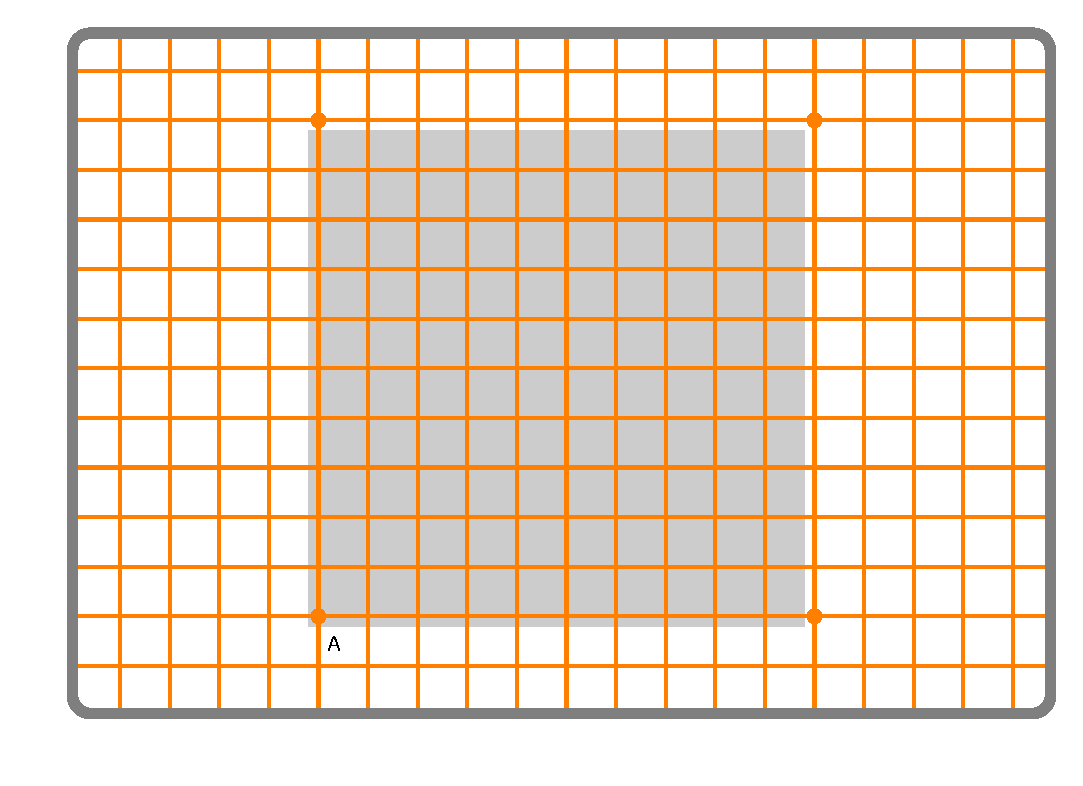
\includegraphics[width=100mm]{flat-torus-1.eps}
  \caption{A flat torus}
  \label{\numb section 7.\numb fig 1}
\end{figure}

The {\small\tt\verm{tag}::spin} in the constructor {\small\verm{Mesh} \azul{torus}}
provides no specific information, it just warns {\maniFEM} that we are on a quotient manifold
and that it must take spins into account.
Specific information about spins is included in the two segments {\small\tt seg\_\,horiz}
and {\small\tt seg\_\,vert}.

This quotient torus is a Riemann manifold with no curvature; it is locally Euclidian
(that is, locally isometric to open sets of $ \mathbb{R}^2 $); we may call it ``flat torus''.
It cannot be embedded in $ \mathbb{R}^3 $, much less be represented graphically.
An unfolded mesh in $ \mathbb{R}^2 $ can be represented graphically,
as in figure \ref{\numb section 7.\numb fig 1}, where vertices and segments from the torus
are drawn more than once.

In figure \ref{\numb section 7.\numb fig 1} we have added a shadow representing
the periodicity cell $ [0,1]^2 $.
This gives a hint about the repeated structure of the the unfolded mesh.
We see that, for instance, the vertex {\small\tt A} shows up four times.
Each segment originating from {\small\tt A} is also drawn four times.
Other vertices and segments are drawn only twice, or only once.
These numbers depend on the position of the vertex or segment and on the size of the
viewing window.

The mesh {\small\tt torus} has 100 squares, 200 segments and 100 vertices.
It has no boundary, it is closed in itself, it covers entirely $ \mathbb{R}^2/{\mathbb Z}^2 $
which is a compact manifold with no boundary.
In contrast, if we mesh the square $ [0,1]^2 $ in the usual Euclidian plane
we get a mesh with 100 squares, 220 segments and 121 vertices (and of course we get a boundary).

Figure \ref{\numb section 7.\numb fig 1} is rather dull because the mesh is very regular.
In paragraphs {\numb section 7.\numb parag 6} -- {\numb section 7.\numb parag 9}
we have introduced an inhomogeneity (a small hole) in the mesh
in order to turn the repetitive pattern more visible.

If you feel uncomfortable with this minimalist approach (of defining a square with only one
vertex), you may think in terms of four squares instead :

\begin{Verbatim}[commandchars=\\\{\},formatcom=\small\tt,
   baselinestretch=0.94,framesep=2mm                      ]
   \verm{Cell} \azul{A} ( \verm{tag}::vertex );  x(A) = 0. ;  y(A) = 0. ;
   \verm{Cell} \azul{B} ( \verm{tag}::vertex );  x(B) = 0.5;  y(B) = 0. ;
   \verm{Cell} \azul{C} ( \verm{tag}::vertex );  x(C) = 0.5;  y(C) = 0.5;
   \verm{Cell} \azul{D} ( \verm{tag}::vertex );  x(D) = 0. ;  y(D) = 0.5;
   
   \verm{Mesh} \azul{AB} ( \verm{tag}::segment, A.reverse(), B, \verm{tag}::divided_in, 5 ),
        \azul{BC} ( \verm{tag}::segment, B.reverse(), C, \verm{tag}::divided_in, 5 ),
        \azul{CD} ( \verm{tag}::segment, C.reverse(), D, \verm{tag}::divided_in, 5 ),
        \azul{DA} ( \verm{tag}::segment, D.reverse(), A, \verm{tag}::divided_in, 5 ),
        \azul{BA1} ( \verm{tag}::segment, B.reverse(), A, \verm{tag}::divided_in, 5, \verm{tag}::spin, g_horiz ),
        \azul{CD1} ( \verm{tag}::segment, C.reverse(), D, \verm{tag}::divided_in, 5, \verm{tag}::spin, g_horiz ),
        \azul{CB2} ( \verm{tag}::segment, C.reverse(), B, \verm{tag}::divided_in, 5, \verm{tag}::spin, g_vert ),
        \azul{DA2} ( \verm{tag}::segment, D.reverse(), A, \verm{tag}::divided_in, 5, \verm{tag}::spin, g_vert );

   \verm{Mesh} \azul{sq1} ( \verm{tag}::rectangle, AB, BC, CD, DA ),
        \azul{sq2} ( \verm{tag}::rectangle, BA1, DA.reverse(), CD1.reverse(), BC.reverse(), \verm{tag}::spin ),
        \azul{sq3} ( \verm{tag}::rectangle, DA2.reverse(), CD.reverse(), CB2, AB.reverse(), \verm{tag}::spin ),
        \azul{sq4} ( \verm{tag}::rectangle, CD1, DA2, BA1.reverse(), CB2.reverse(), \verm{tag}::spin );
	
   \verm{Mesh} \azul{torus} ( \verm{tag}::join, sq1, sq2, sq3, sq4 );
\end{Verbatim}


          %--------------%
\section{~~A curved torus}\label{\numb section 7.\numb parag 5}
          %--------------%

We are now in a position to resume the example in paragraph \ref{\numb section 2.\numb parag 16},
this time by using the quotient manifold $ \mathbb{R}^2/{\mathbb Z}^2 $ introduced in paragraph
\ref{\numb section 7.\numb parag 4}.

\begin{Verbatim}[commandchars=\\\{\},formatcom=\small\tt,frame=single,
   label=parag-\ref{\numb section 7.\numb parag 5}.cpp,rulecolor=\color{coment},
   baselinestretch=0.94,framesep=2mm                                            ]
   \verm{Manifold} \azul{RR2} ( \verm{tag}::Euclid, \verm{tag}::of_dim, 2 );
   \verm{Function} \azul{ab} = RR2.build_coordinate_system ( \verm{tag}::Lagrange, \verm{tag}::of_degree, 1 );
   \verm{Function} \azul{alpha} = ab[0], \azul{beta} = ab[1];
   const double \azul{pi} = 3.1415926536;
   \verm{Function}::Action \azul{g1} ( \verm{tag}::transforms, ab, \verm{tag}::into, (alpha+2.*pi) && beta );
   \verm{Function}::Action \azul{g2} ( \verm{tag}::transforms, ab, \verm{tag}::into, alpha && (beta+2.*pi) );
   \verm{Manifold} \azul{torus_manif} = RR2.quotient ( g1, g2 );

   \verm{Cell} \azul{A} ( \verm{tag}::vertex );  alpha(A) = 0.;  beta(A) = 0.;
   \verm{Mesh} \azul{seg_horiz} ( \verm{tag}::segment, A.reverse(), A,
                    \verm{tag}::divided_in, 40, \verm{tag}::spin, g1 );
   \verm{Mesh} \azul{seg_vert}  ( \verm{tag}::segment, A.reverse(), A,
                    \verm{tag}::divided_in, 20, \verm{tag}::spin, g2 );
   \verm{Mesh} \azul{torus} ( \verm{tag}::rectangle, seg_horiz, seg_vert,
                seg_horiz.reverse(), seg_vert.reverse(), \verm{tag}::spin );

   \cinza{// parametrize the doughnut}
   const double \azul{big_radius} = 3., \azul{small_radius} = 1.;
   \cinza{// define x, y and z as functions of alpha and beta}
   \verm{Function} \azul{x} = ( big_radius + small_radius*\verm{cos}(beta) ) * \verm{cos}(alpha),
            \azul{y} = ( big_radius + small_radius*\verm{cos}(beta) ) * \verm{sin}(alpha),
            \azul{z} = small_radius*\verm{sin}(beta);

   \cinza{// forget about alpha and beta :}
   torus_manif.set_coordinates ( x && y && z );
   \cinza{// in future statements (e.g. for graphical representation)}
   \cinza{// x, y and z will be used, not alpha nor beta :}
   torus.export_msh (\verde{"torus.msh"});
\end{Verbatim}


          %------------------------%
\section{~~A flat torus with a hole}\label{\numb section 7.\numb parag 6}
          %------------------------%

In this paragraph, we perforate the flat torus.
This small inhomogeneity makes the drawing more meaningful.
We also change the shape of the viewing window, just for the fun of it.

\begin{Verbatim}[commandchars=\\\{\},formatcom=\small\tt,frame=single,
   label=parag-\ref{\numb section 7.\numb parag 6}.cpp,rulecolor=\color{coment},
   baselinestretch=0.94,framesep=2mm                                            ]
   std::vector < \verm{Cell} > \azul{vec};
   \verm{CellIterator} \azul{it} = torus.iterator
      ( \verm{tag}::over_cells, \verm{tag}::of_dim, 2, \verm{tag}::around, A );
   for ( it.reset(); it.in_range(); it++ ) vec.push_back ( *it );
   std::vector<\verm{Cell}>::iterator \azul{itv};
   for ( itv = vec.begin(); itv != vec.end(); itv++ )
   \{  \verm{Cell} \azul{sq} = *itv;  sq.remove_from_mesh ( torus );  \}

   torus.draw_ps ( "torus.eps", \verm{tag}::unfold,
                   \verm{tag}::over_region, x*x + 2.*y*y < 3.5 );
\end{Verbatim}

\begin{figure}[ht] \centering
  \psfrag{A}{\tt\textcolor{textindraw}{A}}
  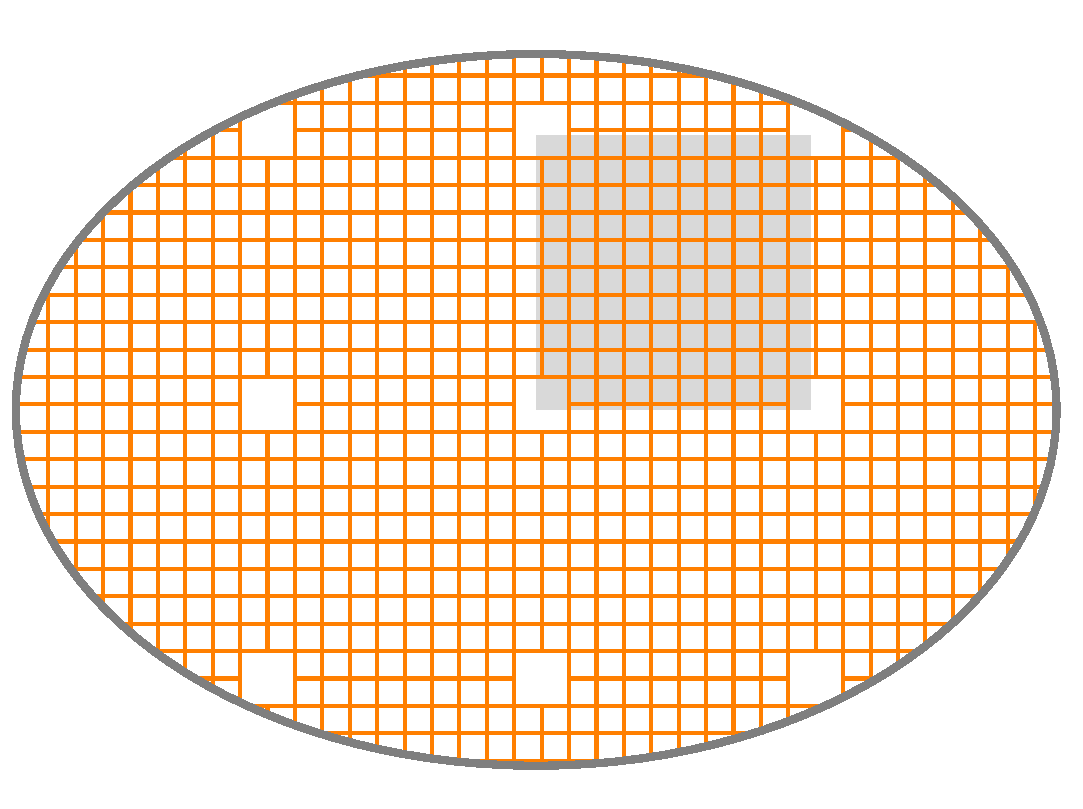
\includegraphics[width=110mm]{flat-torus-2.eps}
  \caption{A flat torus with a hole}
  \label{\numb section 7.\numb fig 2}
\end{figure}

Paragraph \ref{\numb section 9.\numb parag 8} describes iterators around a vertex.

We stress that this mesh has only one hole; figure \ref{\numb section 7.\numb fig 2}
shows several images of the same hole, due to the unfolding.


          %-----------------%
\section{~~A skew flat torus}\label{\numb section 7.\numb parag 7}
          %-----------------%

We can build a skew torus by simply choosing other actions on {\small\tt RR2}.

\begin{Verbatim}[commandchars=\\\{\},formatcom=\small\tt,frame=single,
   label=parag-\ref{\numb section 7.\numb parag 7}.cpp,rulecolor=\color{coment},
   baselinestretch=0.94,framesep=2mm                                            ]
   \verm{Function}::Action \azul{g1} ( tag::transforms, xy, tag::into, (x+1.) && (y+0.1) );
   \verm{Function}::Action \azul{g2} ( tag::transforms, xy, tag::into, (x+0.1) && (y+1.) );
   \verm{Manifold} \azul{torus_manif} = RR2.quotient ( g1, g2 );
\end{Verbatim}

\begin{figure}[ht] \centering
  \psfrag{A}{\tt\textcolor{textindraw}{A}}
  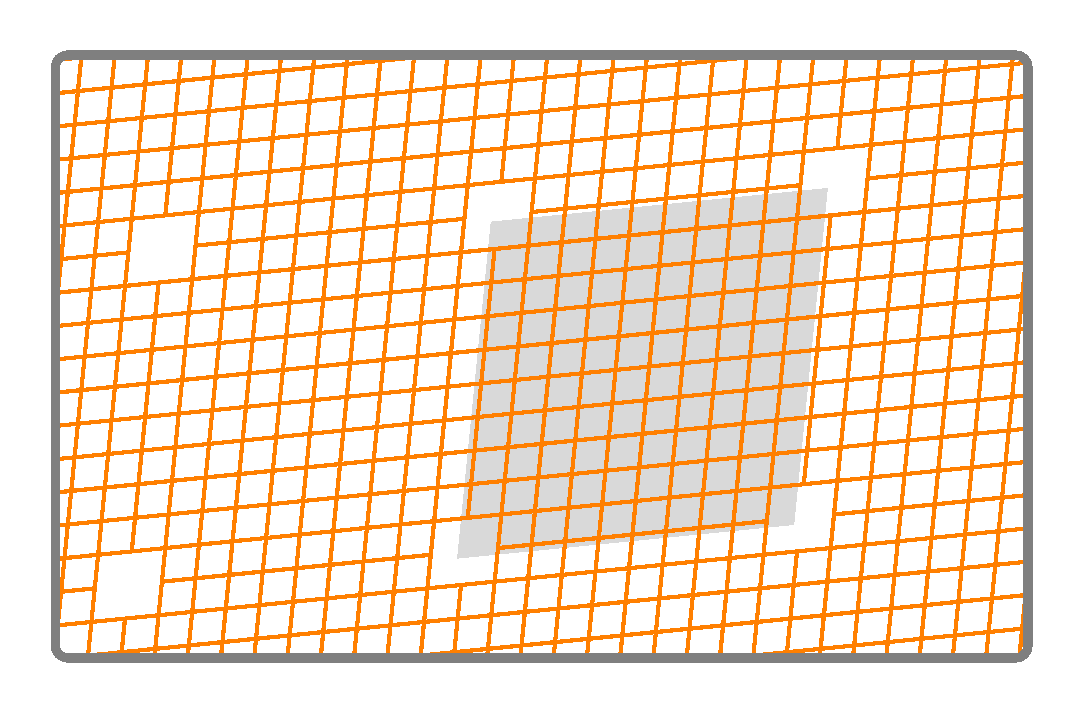
\includegraphics[width=95mm]{flat-torus-3.eps}
  \caption{A skew flat torus}
  \label{\numb section 7.\numb fig 3}
\end{figure}

Again, we have added a shadow representing the periodicity cell, this time a parallelogram.


          %-------------------%
\section{~~A skew torus, again}\label{\numb section 7.\numb parag 8}
          %-------------------%

Here is a different example of a skew torus, this time meshed with squares
rather than skew parallelograms.

\begin{Verbatim}[commandchars=\\\{\},formatcom=\small\tt,frame=single,
   label=parag-\ref{\numb section 7.\numb parag 8}.cpp,rulecolor=\color{coment},
   baselinestretch=0.94,framesep=2mm                                            ]
   \verm{Function}::Action \azul{g1} ( \verm{tag}::transforms, xy, \verm{tag}::into, (x+1.) && y ),
                    \azul{g2} ( \verm{tag}::transforms, xy, \verm{tag}::into, (x+0.5) && (y+1.) );
   \verm{Manifold} \azul{torus_manif} = RR2.quotient ( g1, g2 );

   \verm{Cell} \azul{A} ( \verm{tag}::vertex );  x(A) = 0. ;  y(A) = 0.;
   \verm{Cell} \azul{B} ( \verm{tag}::vertex );  x(B) = 0.5;  y(B) = 0.;

   \verm{Mesh} \azul{AB} ( \verm{tag}::segment, A.reverse(), B, \verm{tag}::divided_in, 5 );
   \verm{Mesh} \azul{BA1} ( \verm{tag}::segment, B.reverse(), A, \verm{tag}::divided_in, 5, \verm{tag}::spin, g1 );
   \verm{Mesh} \azul{BA2} ( \verm{tag}::segment, B.reverse(), A, \verm{tag}::divided_in, 10, \verm{tag}::spin, g2 );
   \verm{Mesh} \azul{AB2} ( \verm{tag}::segment, A.reverse(), B, \verm{tag}::divided_in, 10, \verm{tag}::spin, g2-g1 );

   \verm{Mesh} \azul{sq1} ( \verm{tag}::rectangle, AB, BA2, BA1.reverse(), AB2.reverse(), \verm{tag}::spin );
   \verm{Mesh} \azul{sq2} ( \verm{tag}::rectangle, BA2.reverse(), BA1, AB2, AB.reverse(), \verm{tag}::spin );

   \verm{Mesh} \azul{torus} ( \verm{tag}::join, sq1, sq2 );
\end{Verbatim}


\begin{figure}[ht] \centering
  \psfrag{A}{\tt\textcolor{textindraw}{A}}
  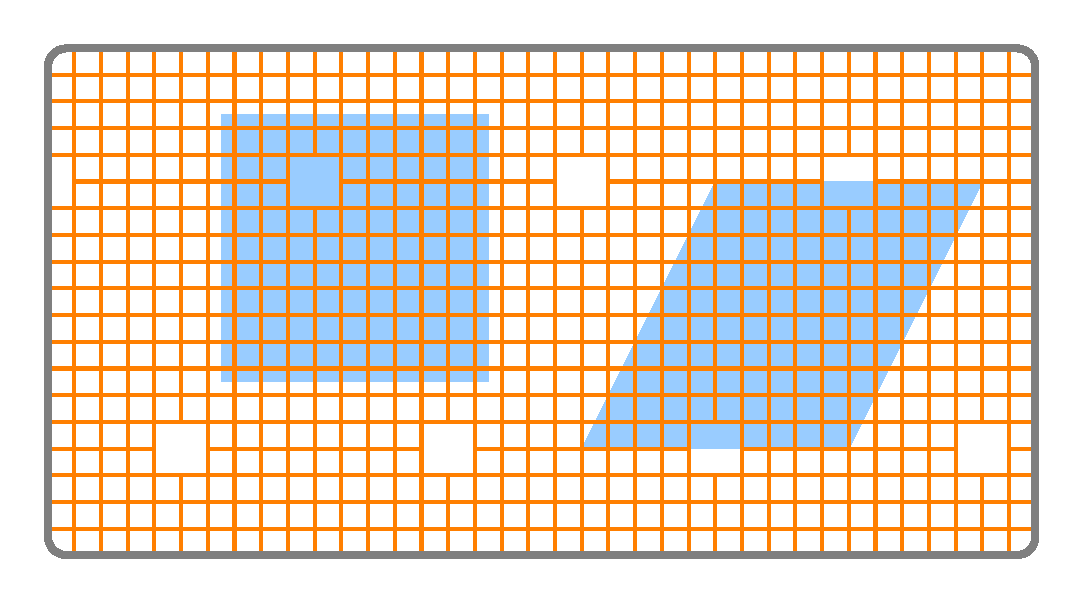
\includegraphics[width=130mm]{flat-torus-4.eps}
  \caption{A different torus}
  \label{\numb section 7.\numb fig 4}
\end{figure}

In figure \ref{\numb section 7.\numb fig 4} we have drawn two shadows.
The skew shadow can be called ``periodicity cell''; we call the other one ``representative domain''.


          %------------------------%
\section{~~Using triangular patches}\label{\numb section 7.\numb parag 9}
          %------------------------%

Here is an example of a torus built with two triangular patches.

\begin{figure}[ht] \centering
  \psfrag{A}{\tt\textcolor{textindraw}{A}}
  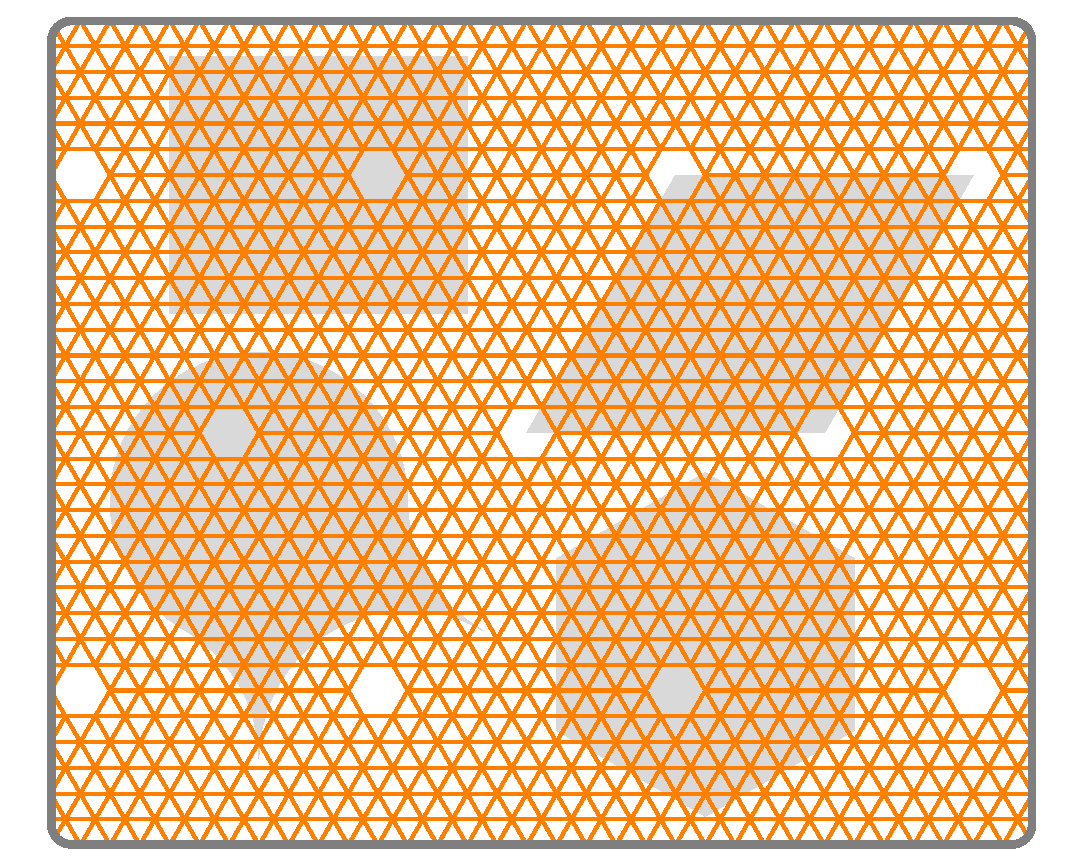
\includegraphics[width=130mm]{flat-torus-5.eps}
  \caption{A torus built with triangles}
  \label{\numb section 7.\numb fig 5}
\end{figure}

\begin{Verbatim}[commandchars=\\\{\},formatcom=\small\tt,frame=single,
   label=parag-\ref{\numb section 7.\numb parag 9}.cpp,rulecolor=\color{coment},
   baselinestretch=0.94,framesep=2mm                                            ]
   \verm{Function}::Action \azul{g1} ( \verm{tag}::transforms, xy, \verm{tag}::into, (x+1.) && y ),
                    \azul{g2} ( \verm{tag}::transforms, xy, \verm{tag}::into, (x+0.5) && (y+0.866) );
   \verm{Manifold} \azul{torus_manif} = RR2.quotient ( g1, g2 );

   \verm{Cell} \azul{A} ( \verm{tag}::vertex );  x(A) = 0.;  y(A) = 0.;

   \verm{Mesh} \azul{seg_horiz} ( \verm{tag}::segment, A.reverse(), A,
                    \verm{tag}::divided_in, 10, \verm{tag}::spin, g1 ),
        \azul{seg1}      ( \verm{tag}::segment, A.reverse(), A,
                    \verm{tag}::divided_in, 10, \verm{tag}::spin, g2 ),
        \azul{seg2}      ( \verm{tag}::segment, A.reverse(), A,
                    \verm{tag}::divided_in, 10, \verm{tag}::spin, g2-g1 );

   \verm{Mesh} \azul{tri1} ( \verm{tag}::triangle, seg_horiz, seg2, seg1.reverse(), \verm{tag}::spin ),
        \azul{tri2} ( \verm{tag}::triangle, seg_horiz.reverse(), seg2.reverse(), seg1, \verm{tag}::spin );
   
   \verm{Mesh} \azul{torus} ( \verm{tag}::join, tri1, tri2 );
\end{Verbatim}

In figure \ref{\numb section 7.\numb fig 5} we have drawn four shadows.
The skew paralellogram can be called ``periodicity cell'';
the other ones are ``representative domains''.
Due to the shape of one of these shadows, this periodic arrangement is often called
``hexagonal periodicity''.


          %--------%
\section{~~Exercise}\label{\numb section 7.\numb parag 10}
          %--------%

Build the mesh shown in figure \ref{\numb section 7.\numb fig 5}
(the same as in paragraph \ref{\numb section 7.\numb parag 9}) using only one rectangular patch.
(Hint: have a look at paragraphs \ref{\numb section 2.\numb parag 3} and
\ref{\numb section 2.\numb parag 8}.)


